\section{Converter setup}
\label{sec:setup}

Since the general measurement instrument setup was comparable for most
of the measurements, I decided to collect this setup here for
conciseness. The first experiments used a Longpath-DOAS instrument, as
it allowed for a precise ozone measurement. Afterwards I transferred
to a CE-DOAS instrument, because of its better localisation and
nitrogen oxides detection capabilities.

\subsection{Ozone generator setup}
\label{sec:ozone-setup}

As a proof of concept I built the ozone generator on a wooden board
as can be seen in Figure~\ref{fig:setup}. As described in
Section~\ref{sec:requirements}, the lab air is first filtered and then
sent through an alluminium coated tube containing a Pen-Ray mercury
lamp (Model 11SC-1). It has a lighted length of
\SI{53.8}{\milli\meter} and primary emission band at
\SI{254}{\nano\meter}. The mercury lamp's spectrum is not perfect for
my purpose as its strongest emission is in the ozone dissociation
wavelength range, whereas the lamp has almost no energy output below
the Oxygen dissociation limit (c.\,f.~\cite{lamp}). However, since the
Oxygen concentration in ambient air is so high, I still expect enough
ozone to be produced. In order to make sure that the \ch{N2O} is completely
converted to \ch{NO2}, I introduce a \SI{3}{\meter} teflon
tube. Afterwards the ozone enriched air passes another Silica gel
filter and is then expected to be \ch{NO_x} free.

In order to be able to measure the ozone production after the last filter a
cuvette is added, which can be entered in the light path of a
Longpath-DOAS instrument (cf.\ Fig.~\ref{fig:cuvette}). The length of
the lightpath through the cuvette is \SI{8.7}{\centi\meter}. 

The Pen-Ray power source can switch the current between
\SI{10}{\milli\ampere} and \SI{17}{\milli\ampere}. If not otherwisely
stated the measurements were performed at \SI{10}{\milli\ampere}.
Furthermore the flow $\Phi_{\ch{O 3}}$ can be set via the flowmeter
between \num{0} and \SI{0.3}{\liter\per\minute}. The lowest stable
positive flow is \SI{0.03}{\liter\per\minute}.

\begin{figure}[htbp]
  \centering
  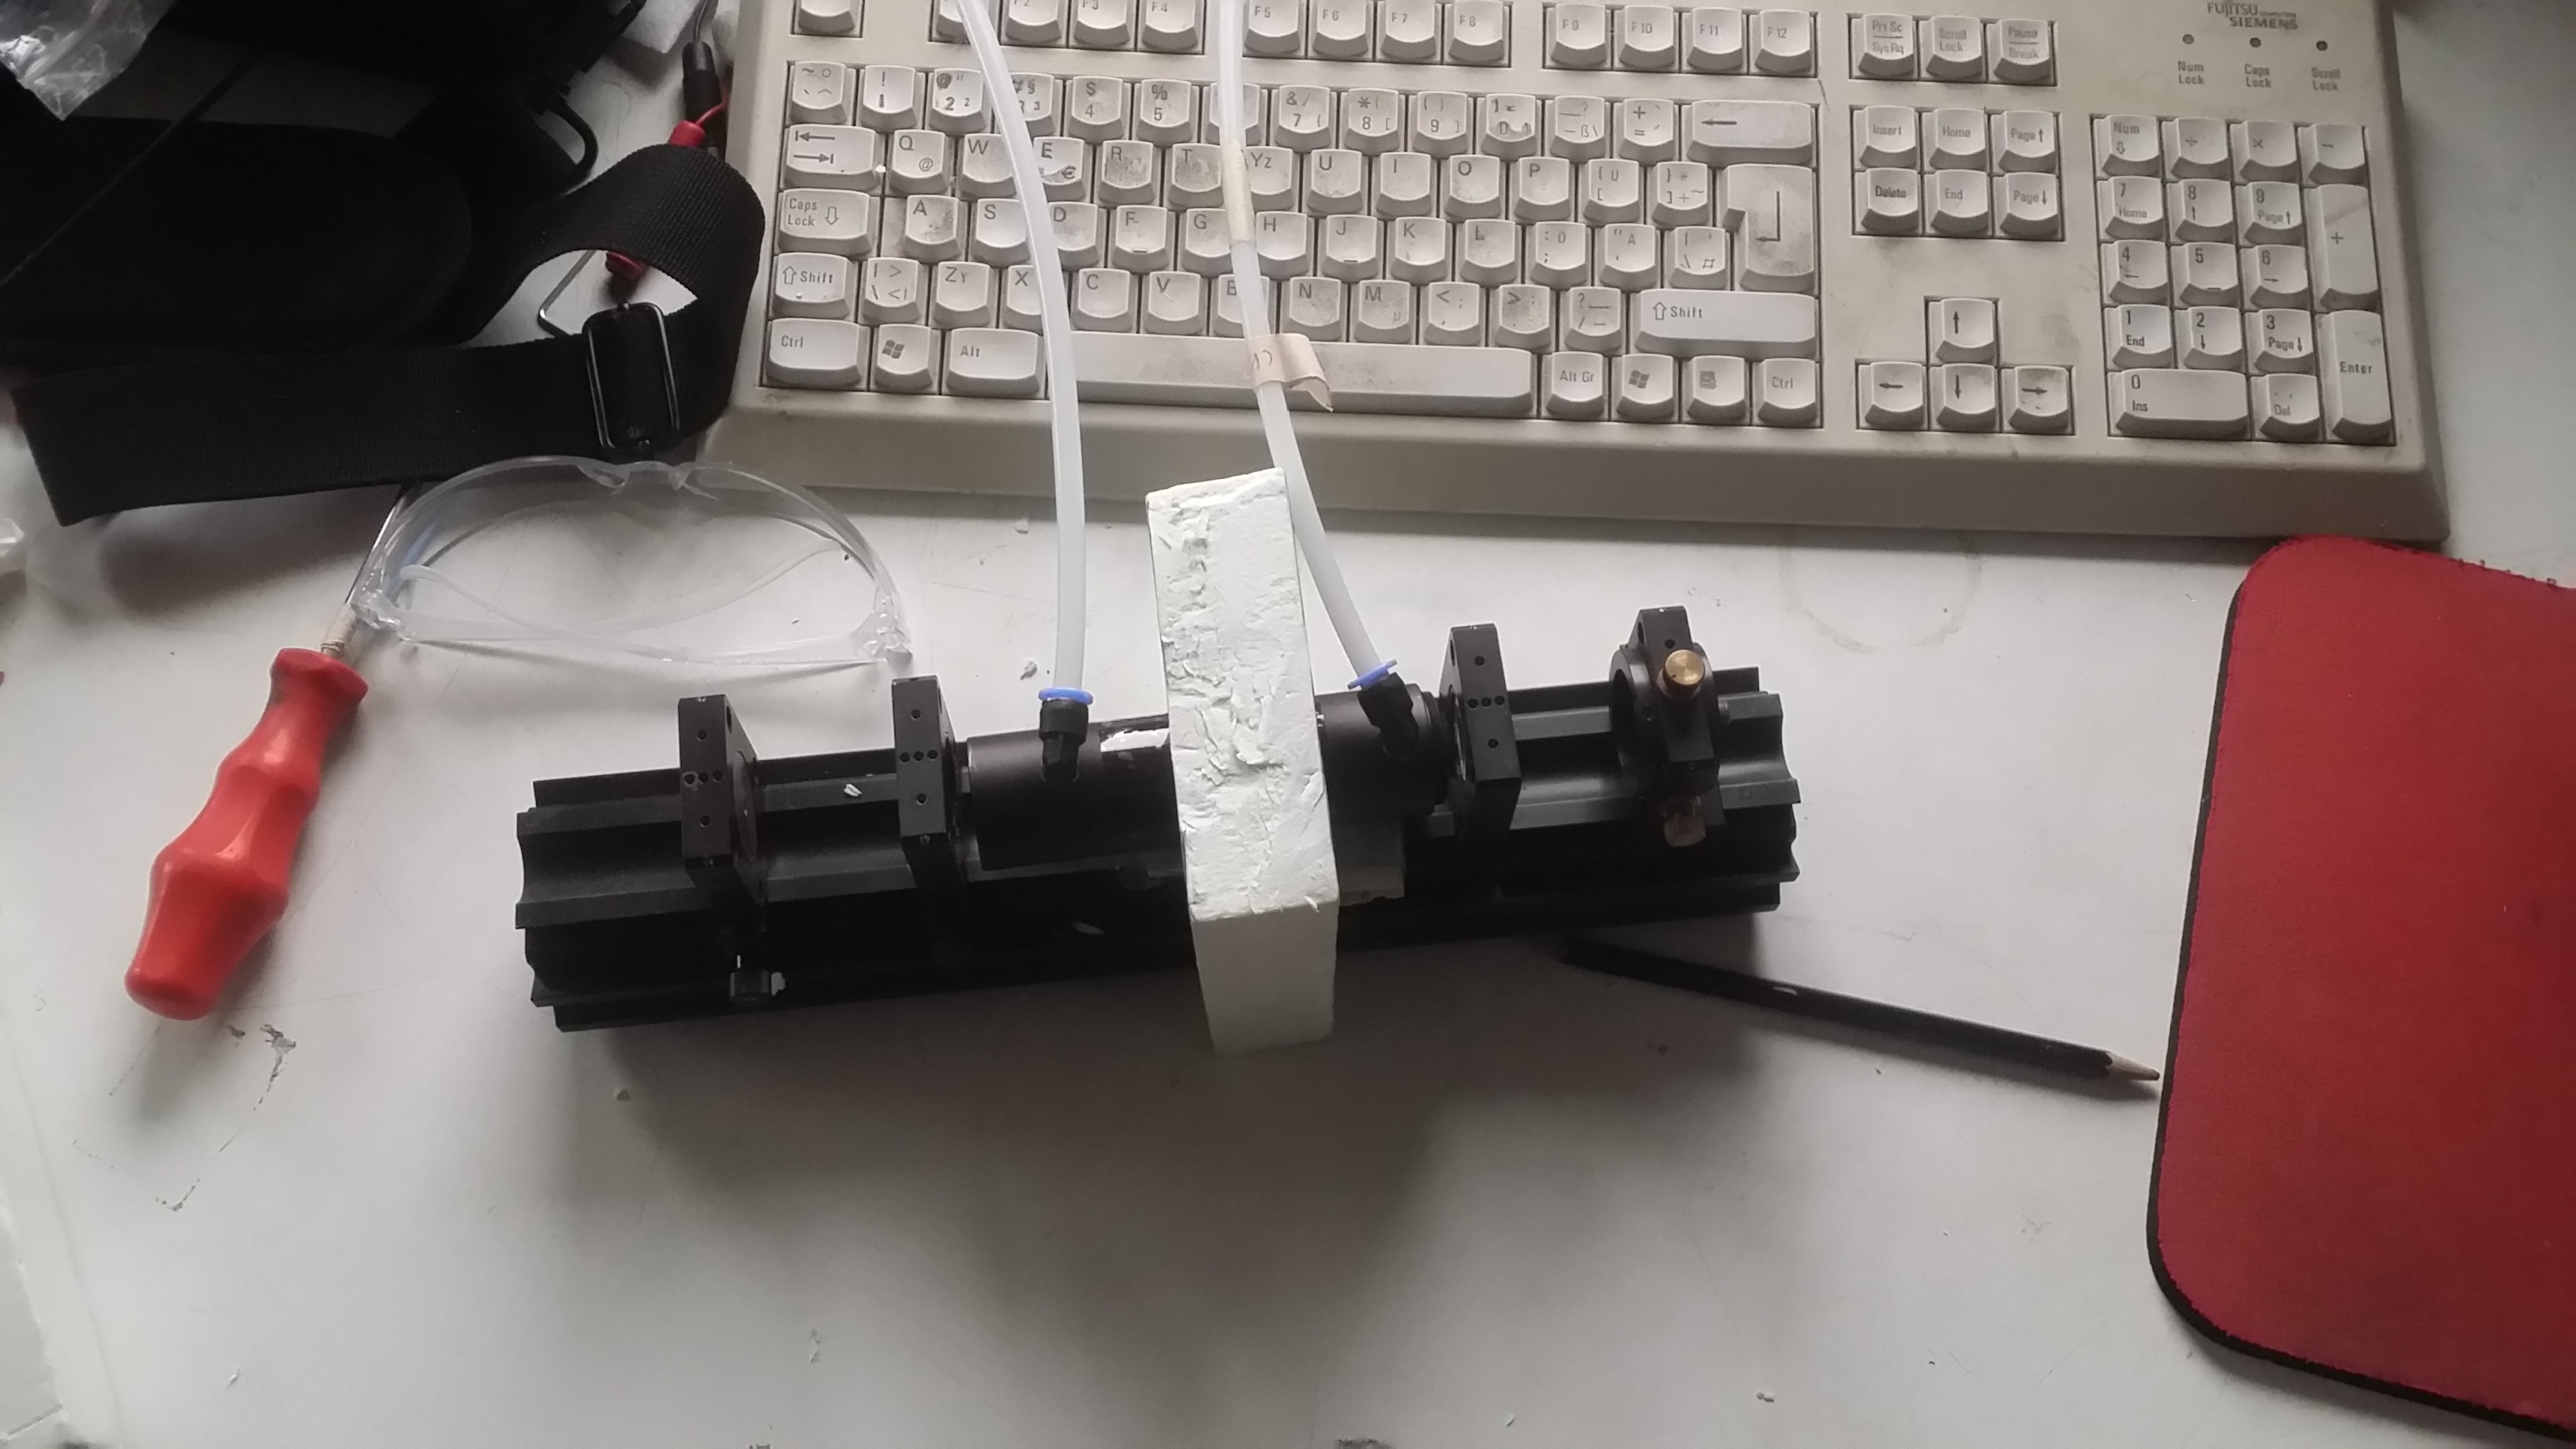
\includegraphics[width=0.7\textwidth]{images/cuvette.jpg}
  \caption{Cuvette together with styrofoam mount on an optical
    rail. The outermost riders are the mounts for the optical
    fibers. The riders within consist of two collimators.}
  \label{fig:cuvette}
\end{figure}

\begin{figure}[htbp]
  \centering
  {
  \def\svgwidth{0.9\linewidth}
  %% Creator: Inkscape inkscape 0.91, www.inkscape.org
%% PDF/EPS/PS + LaTeX output extension by Johan Engelen, 2010
%% Accompanies image file 'setup.pdf_tex.pdf' (pdf, eps, ps)
%%
%% To include the image in your LaTeX document, write
%%   \input{<filename>.pdf_tex}
%%  instead of
%%   \includegraphics{<filename>.pdf}
%% To scale the image, write
%%   \def\svgwidth{<desired width>}
%%   \input{<filename>.pdf_tex}
%%  instead of
%%   \includegraphics[width=<desired width>]{<filename>.pdf}
%%
%% Images with a different path to the parent latex file can
%% be accessed with the `import' package (which may need to be
%% installed) using
%%   \usepackage{import}
%% in the preamble, and then including the image with
%%   \import{<path to file>}{<filename>.pdf_tex}
%% Alternatively, one can specify
%%   \graphicspath{{<path to file>/}}
%% 
%% For more information, please see info/svg-inkscape on CTAN:
%%   http://tug.ctan.org/tex-archive/info/svg-inkscape
%%
\begingroup%
  \makeatletter%
  \providecommand\color[2][]{%
    \errmessage{(Inkscape) Color is used for the text in Inkscape, but the package 'color.sty' is not loaded}%
    \renewcommand\color[2][]{}%
  }%
  \providecommand\transparent[1]{%
    \errmessage{(Inkscape) Transparency is used (non-zero) for the text in Inkscape, but the package 'transparent.sty' is not loaded}%
    \renewcommand\transparent[1]{}%
  }%
  \providecommand\rotatebox[2]{#2}%
  \ifx\svgwidth\undefined%
    \setlength{\unitlength}{1567.76523438bp}%
    \ifx\svgscale\undefined%
      \relax%
    \else%
      \setlength{\unitlength}{\unitlength * \real{\svgscale}}%
    \fi%
  \else%
    \setlength{\unitlength}{\svgwidth}%
  \fi%
  \global\let\svgwidth\undefined%
  \global\let\svgscale\undefined%
  \makeatother%
  \begin{picture}(1,0.56250002)%
    \put(0,0){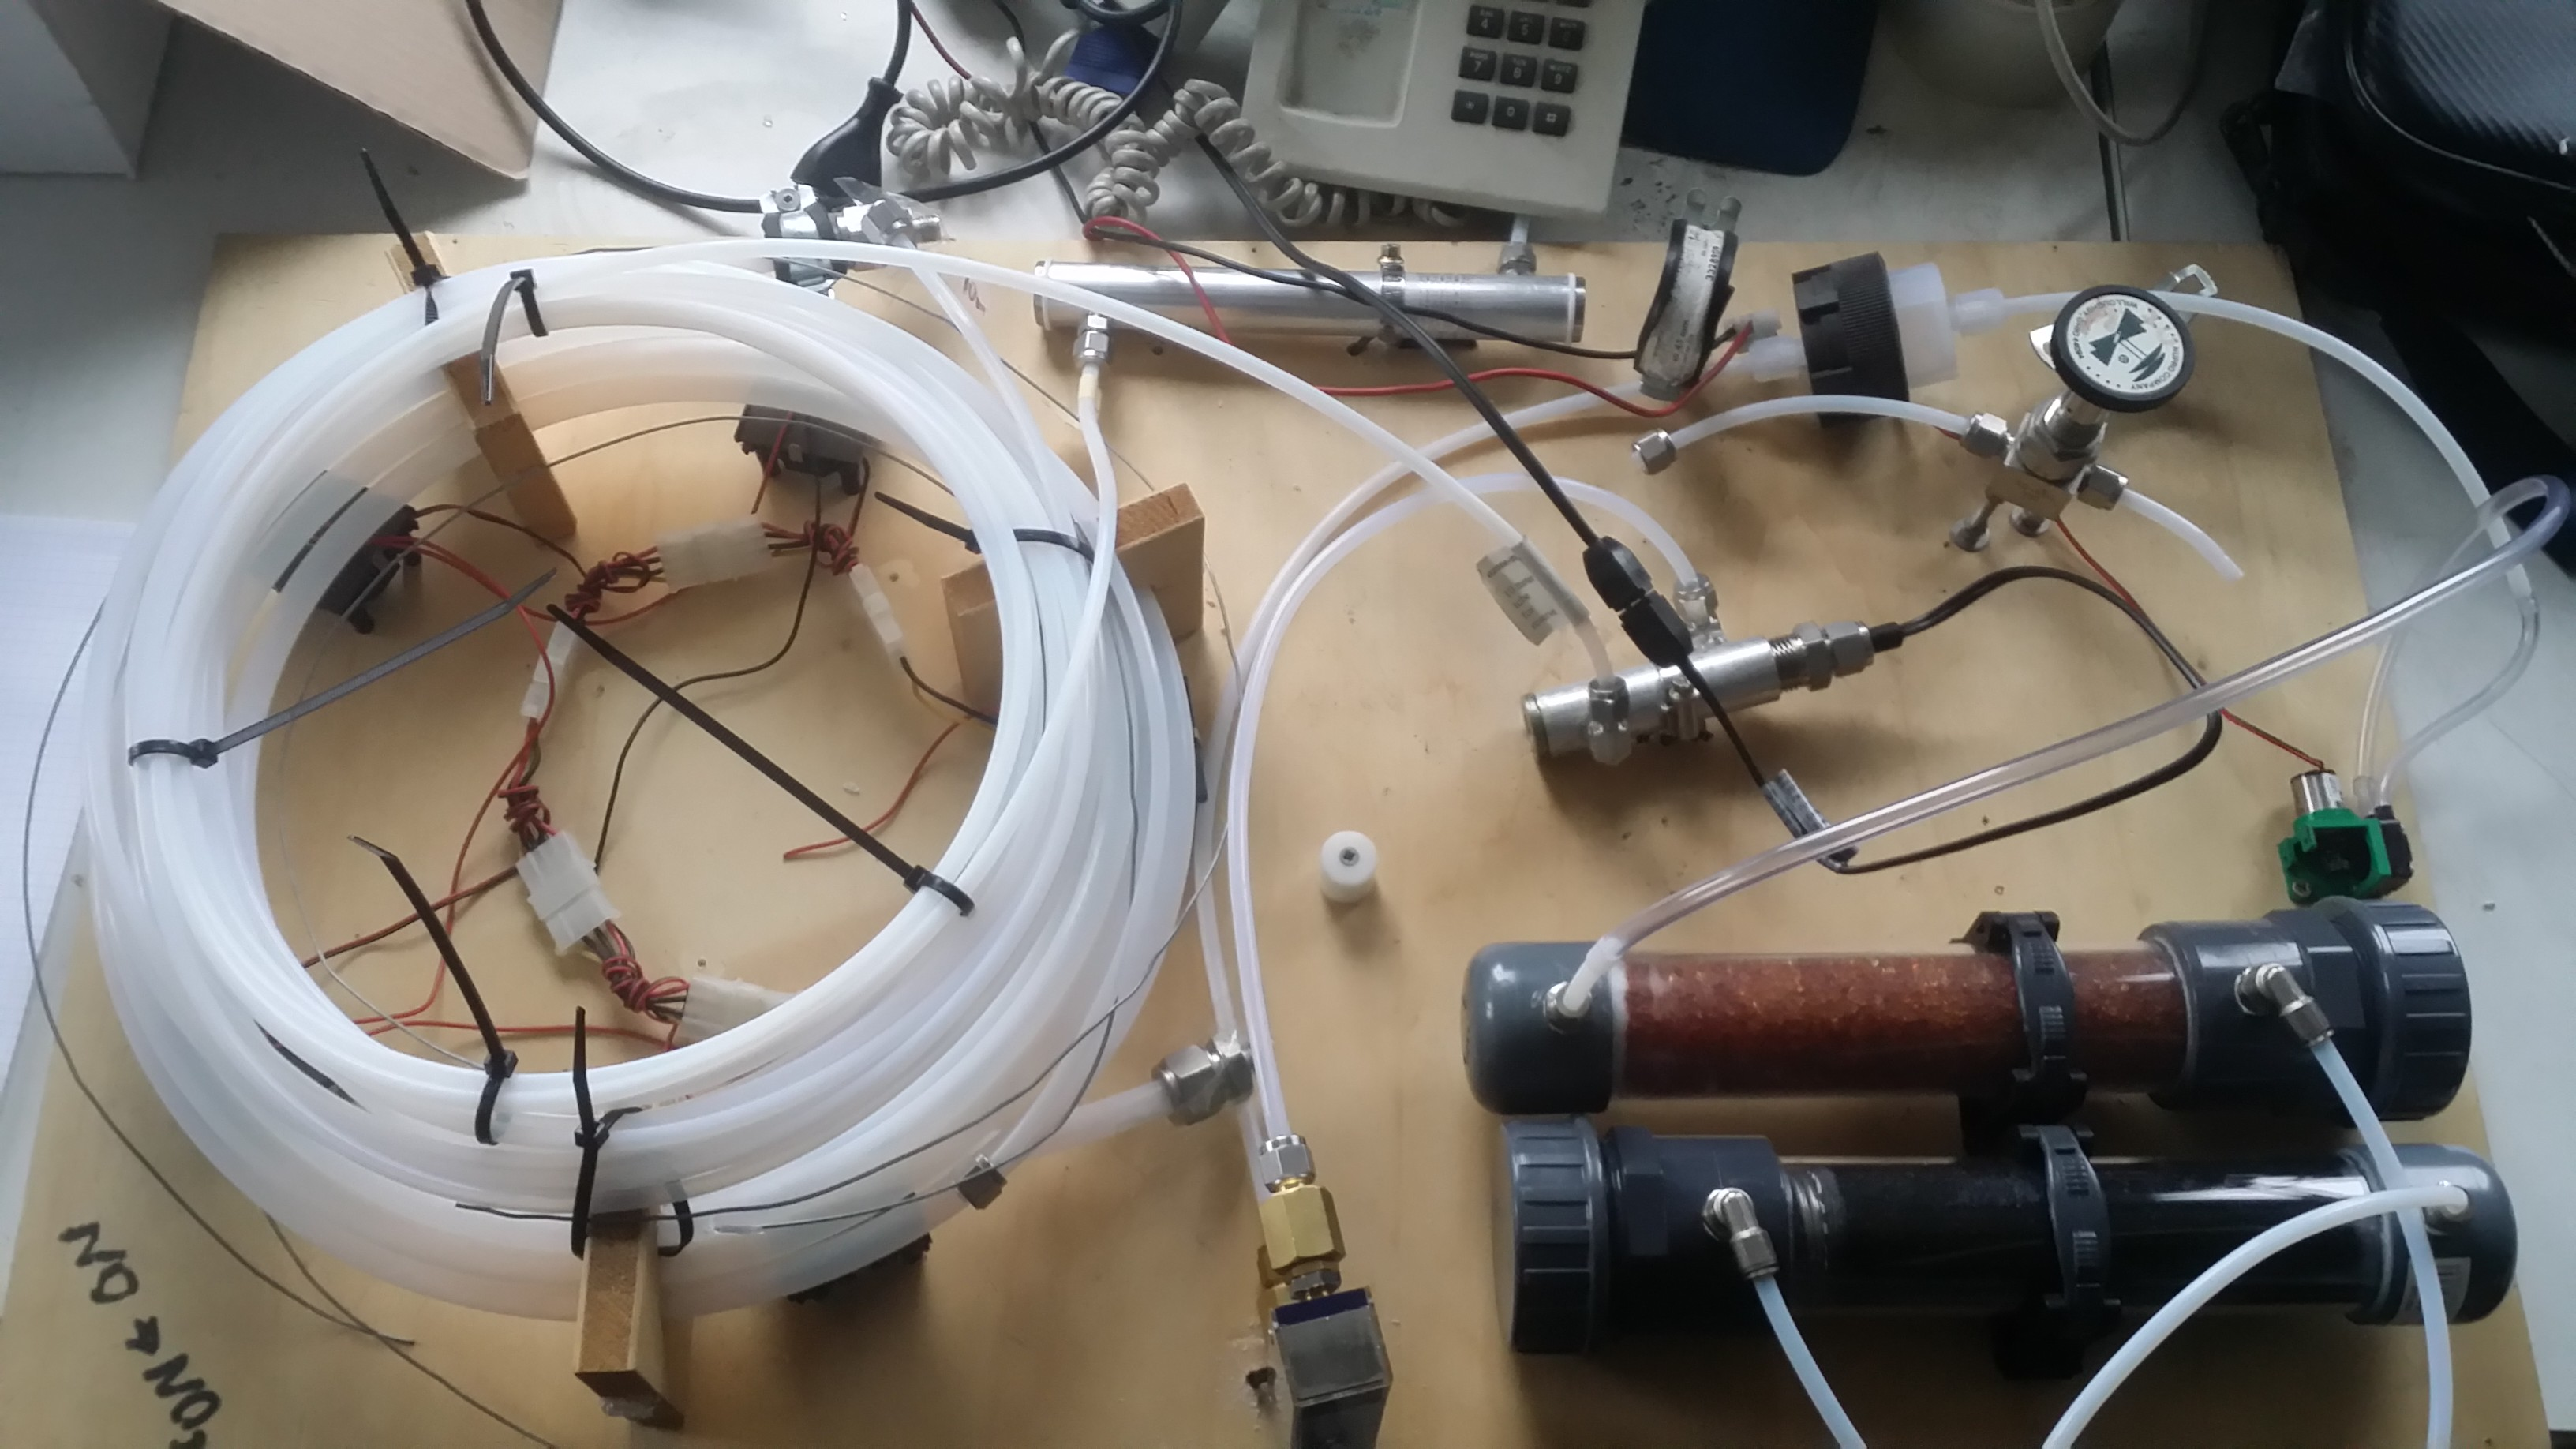
\includegraphics[width=\unitlength,page=1]{setup.pdf}}%
    \put(0.72339254,0.0272422){\color[rgb]{0,0,0}\makebox(0,0)[lb]{carbon filter}}%
    \put(0.68467052,0.20608212){\color[rgb]{0,0,0}\makebox(0,0)[lb]{\smash{silica gel}}}%
    \put(0.84485225,0.27636329){\color[rgb]{0,0,0}\makebox(0,0)[lb]{\smash{pump}}}%
    \put(0.66524548,0.47215208){\color[rgb]{0,0,0}\makebox(0,0)[lb]{\smash{particle filter}}}%
    \put(0.37854499,0.02340413){\color[rgb]{0,0,0}\makebox(0,0)[lb]{\smash{flowmeter}}}%
    \put(0.41093385,0.46876799){\color[rgb]{0,0,0}\makebox(0,0)[lb]{\smash{silica gel in tube}}}%
    \put(0.55474278,0.26558162){\color[rgb]{0,0,0}\makebox(0,0)[lb]{\smash{penray lamp in tube}}}%
    \put(0,0){\includegraphics[width=\unitlength,page=2]{setup.pdf}}%
    \put(1.00286136,0.04729665){\color[rgb]{0,0,0}\makebox(0,0)[lb]{\smash{lab air}}}%
    \put(0.59985726,0.5399915){\color[rgb]{0,0,0}\makebox(0,0)[lb]{\smash{ozone}}}%
    \put(0,0){\includegraphics[width=\unitlength,page=3]{setup.pdf}}%
  \end{picture}%
\endgroup%

%%% Local Variables:
%%% mode: latex
%%% TeX-master: "../Bachelor"
%%% End:

  }
  \phantom{h}\\
  \vspace{2cm}
  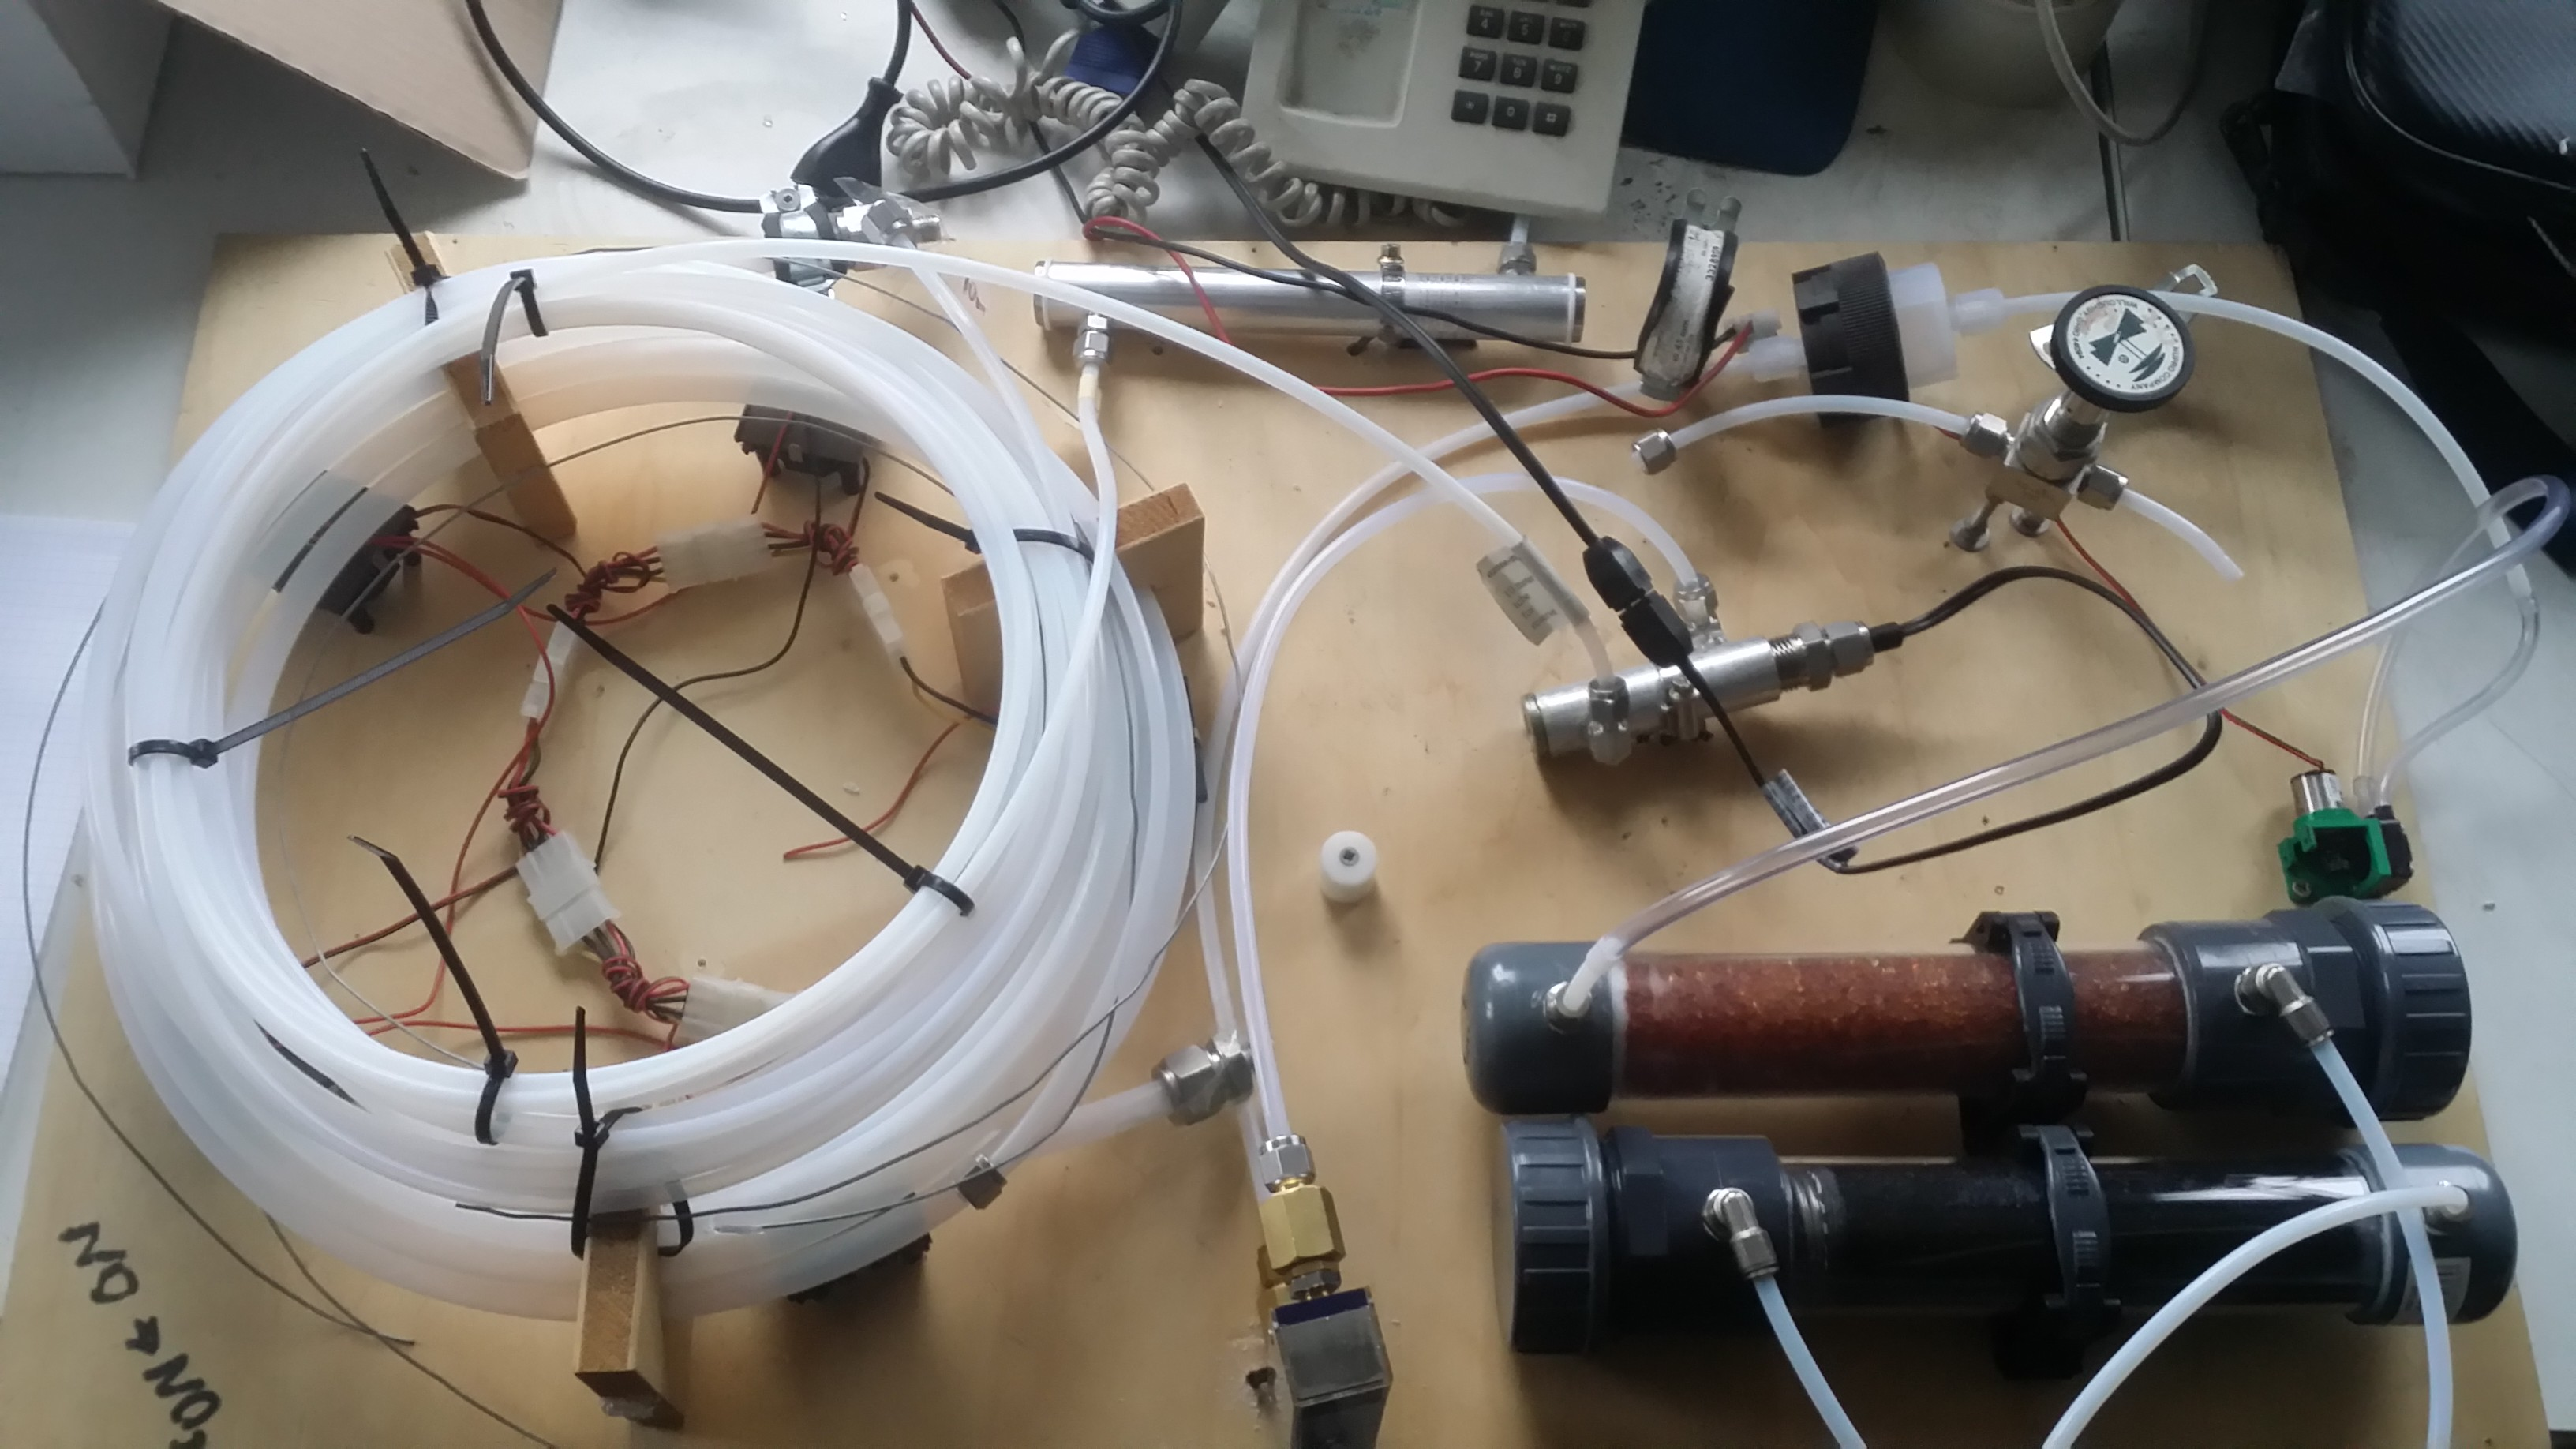
\includegraphics[width=0.9\linewidth]{setup.jpg}
  \caption{ozone generator setup. Schematic and picture.}
  \label{fig:setup}
\end{figure}

The cuvette was entered into the ligthpath of a Longpath-DOAS
instrument (attached to an Amundsen telescope located at the rooftop
laboratory at the IUP building). Since I expected rather high ozone
concentrations, I forewent the advantage of a cavity enhanced
pathlength. The upside of this setup was that the instrument contains
a laser driven light source which together with appropriate filters
emits at a wavelength of $\lambda \approx \SI{290}{\nano\meter}$. As
mentioned in Section~\ref{sec:theory-ozone}, ozone has a strong
absorption cross section in this region, which made it possible to
determine the concentration very precisely. The used spectrograph has
2048 channesl and is calibrated to a wavelength region of \num{268} to
\SI{312}{\nano\meter}.

\subsection{Inclusion into a CE-DOAS instrument}
\label{sec:inclusion}

\begin{figure}[htbp]
  \centering
  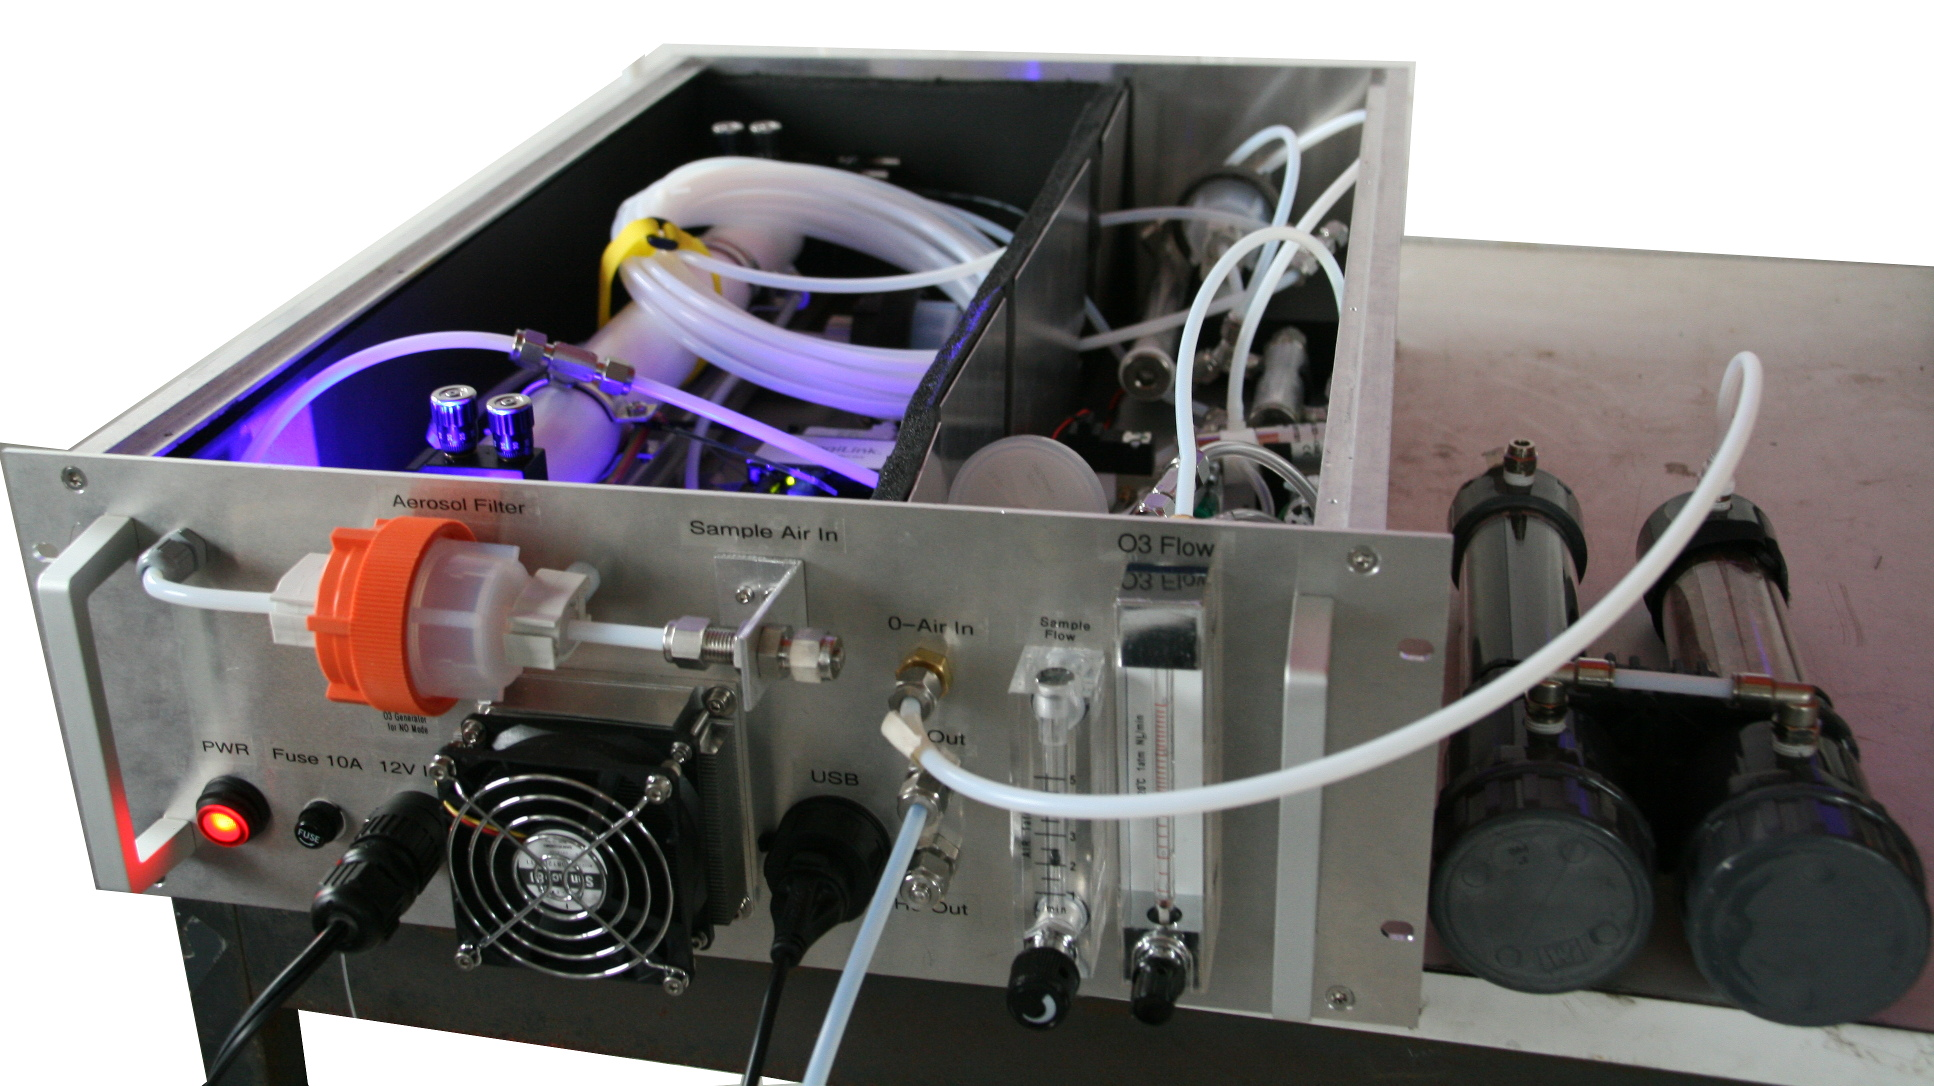
\includegraphics[width=0.8\textwidth]{images/InstrumentEdited_small.jpg}
  \caption{EnviMeS CE-DOAS instrument with \ch{NO} to \ch{NO2}
    converter}
  \label{fig:envimes}
\end{figure}

\begin{figure}[htbp]
  \centering
  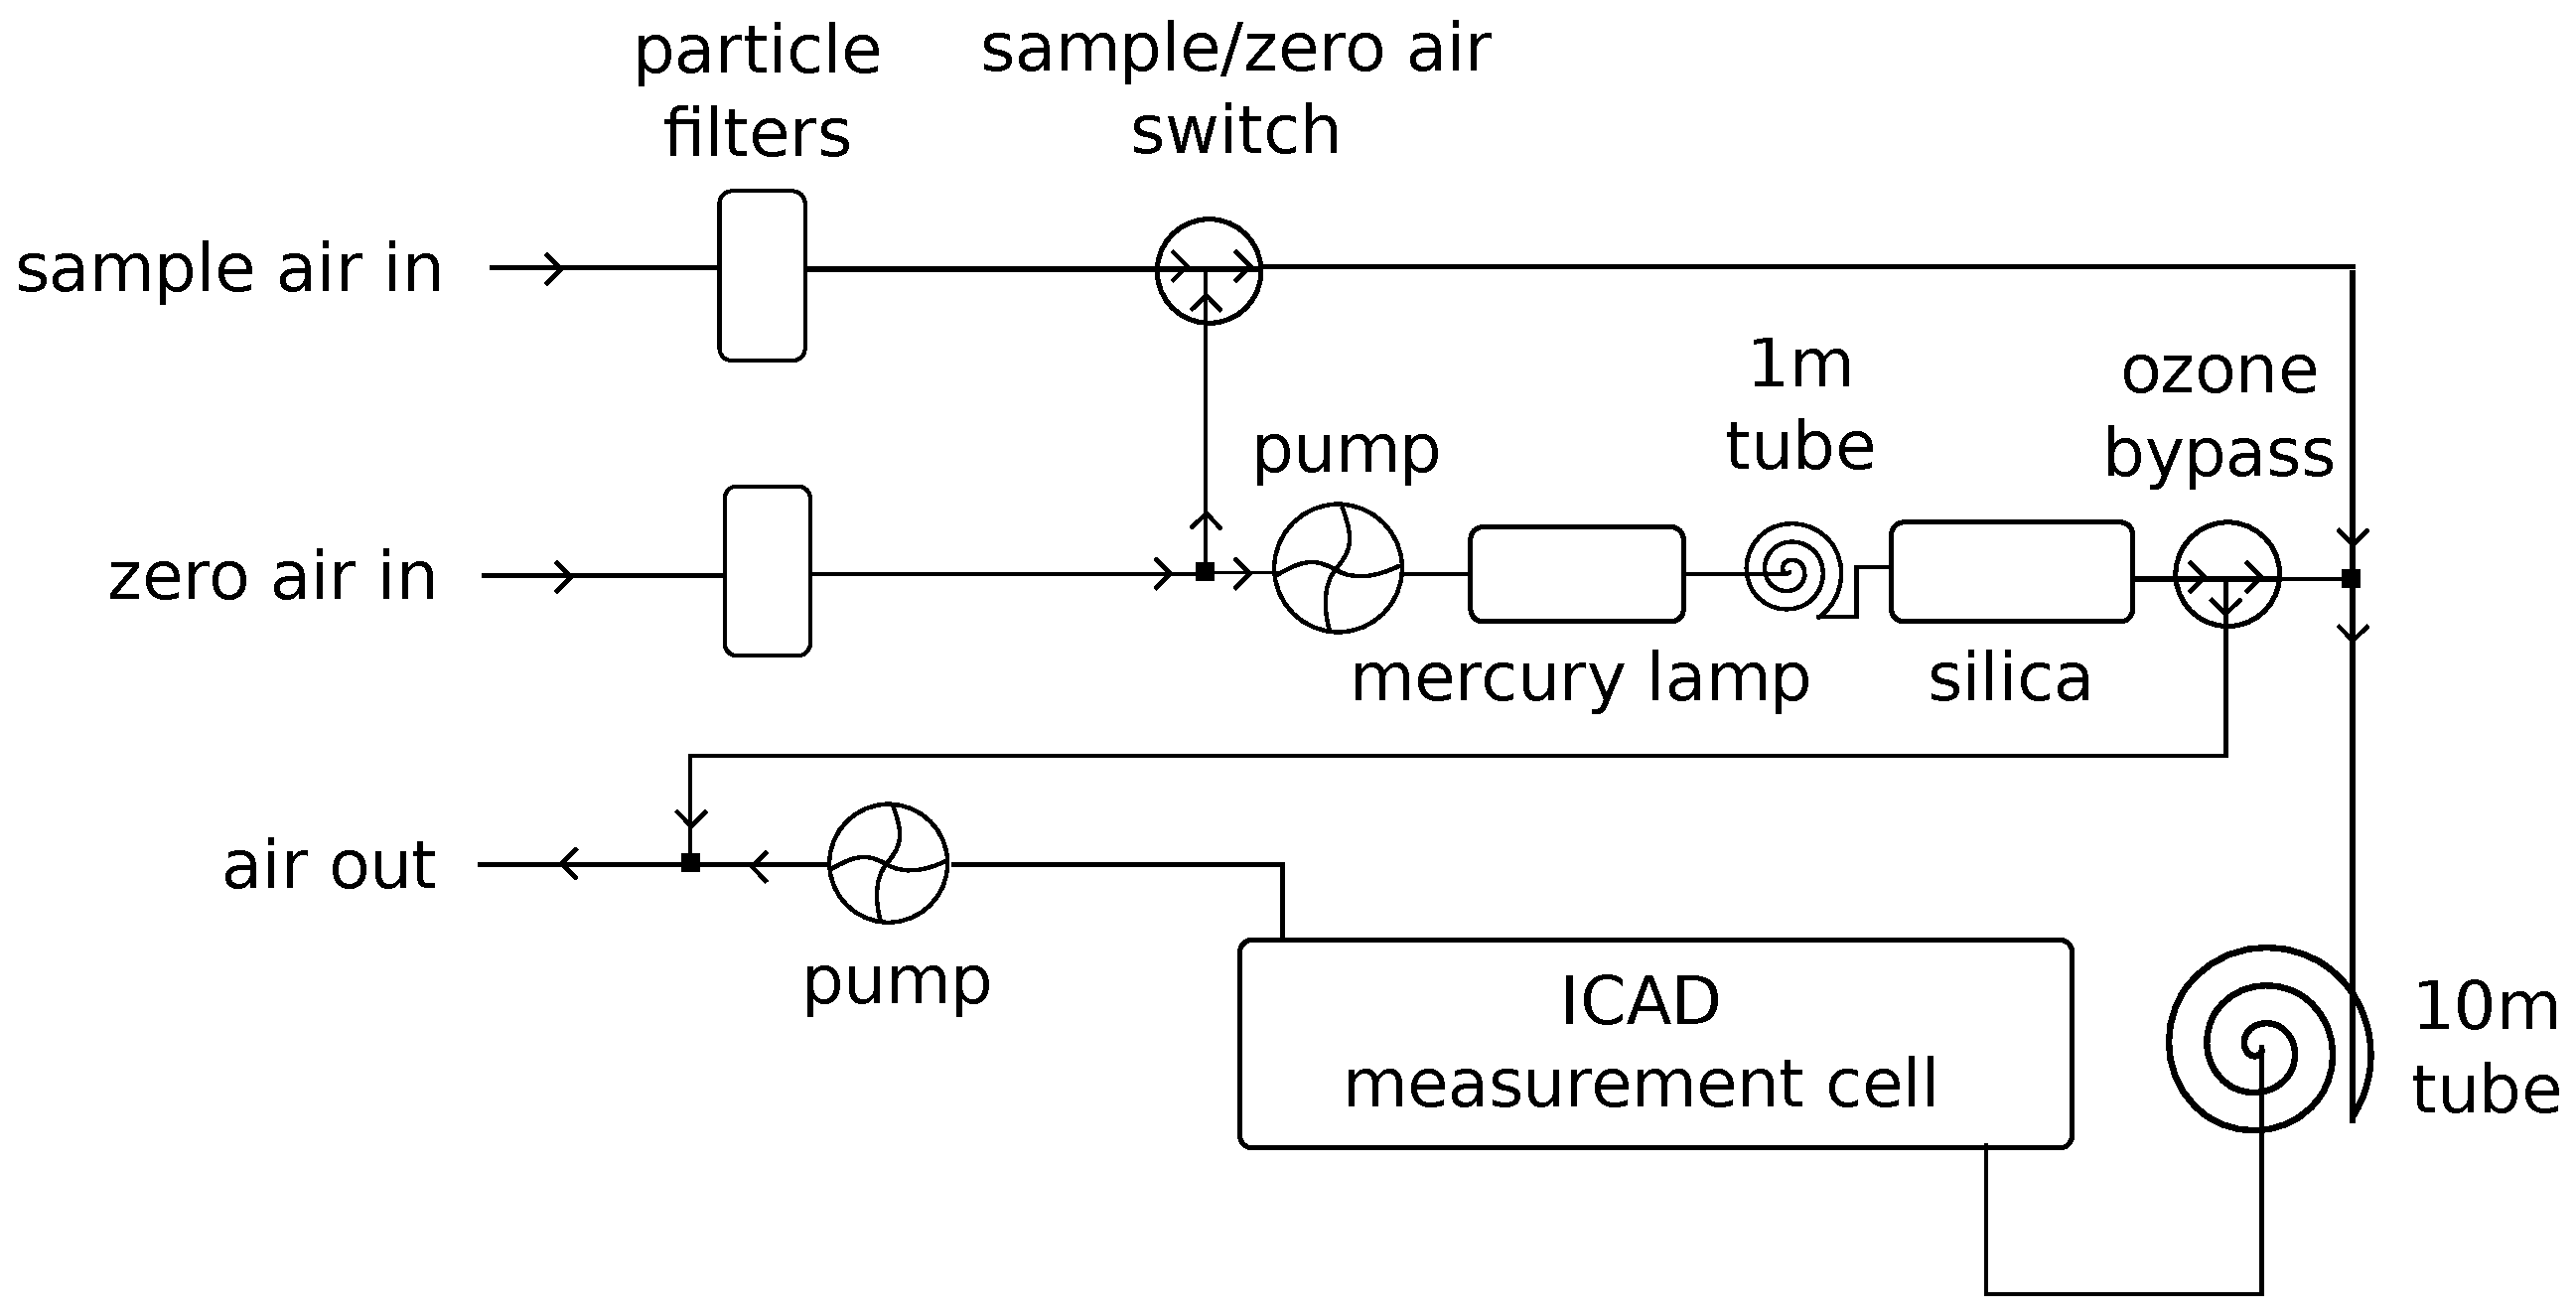
\includegraphics[width=0.8\textwidth]{images/envimes_setup.eps}
  \caption{Schematic of EnviMeS CE-DOAS instrument with \ch{NO} to
    \ch{NO2} converter.}
  \label{fig:envimes-schematic}
\end{figure}

After the above setup was tested the converter was added to an
existing CE-DOAS instrument. The instrument was already supplied with
an \ch{O3} generator, but lacked a Silica gel filter, which was
added. The instrument can be seen in
Figure~\ref{fig:envimes}. Figure~\ref{fig:envimes-schematic} contains
a slightly simplified schematic view of the instrument. Zero air is
used to generate the ozone, since it is already sufficientyl trace gas
free (except for \ch{N2O}). After the mercury lamp there is a
\SI{1}{\meter} reaction path before the silica filter follows. After
that there is an ozone bypass valve, which is operated
electromechanically and allows for the switch between an ozone free and
an ozone enriched air flow in the cavity. The sample air (with or
without ozone) passes a \SI{10}{\meter} reaction path. In later
experiments the length of the reaction path was varied to measure the
influence on the \ch{NO} conversion (c.\,f.\
Sec.~\ref{sec:requirements} for the theory and Sec.~\ref{sec:no} for
measurements). The total flow $\Phi$ can be adapted, but was always
set to \SI{2}{\liter\per\minute}. The ozone flow can be adapted (as
in Sec.~\ref{sec:ozone-setup}) from 0 to
\SI{0.3}{\liter\per\minute}. The lowest stable positive flow is
\SI{0.03}{\liter\per\minute}. To determine the ozone production rate
this flow was varied. When actual \ch{NO} or \ch{NO_x} measurements
were performed the flow was fixed to \SI{0.03}{\liter\per\minute}.

The light source of the instrument is a led with maximum intensity at
$\lambda \approx \SI{444}{\nano\meter}$. The effective pathlength
$L_0$ of the cavity had a maximum at this wavelength of
\SI{1.3}{\kilo\meter}. A plot of the pathlength can be found in
Figure~\ref{fig:pathlength}. The spectrograph has \num{2048} channels
and is calibrated to a wavelength region of \num{395} to
\SI{490}{\nano\meter}.

\begin{figure}[htbp]
  \centering
  % GNUPLOT: LaTeX picture with Postscript
\begingroup
  \makeatletter
  \providecommand\color[2][]{%
    \GenericError{(gnuplot) \space\space\space\@spaces}{%
      Package color not loaded in conjunction with
      terminal option `colourtext'%
    }{See the gnuplot documentation for explanation.%
    }{Either use 'blacktext' in gnuplot or load the package
      color.sty in LaTeX.}%
    \renewcommand\color[2][]{}%
  }%
  \providecommand\includegraphics[2][]{%
    \GenericError{(gnuplot) \space\space\space\@spaces}{%
      Package graphicx or graphics not loaded%
    }{See the gnuplot documentation for explanation.%
    }{The gnuplot epslatex terminal needs graphicx.sty or graphics.sty.}%
    \renewcommand\includegraphics[2][]{}%
  }%
  \providecommand\rotatebox[2]{#2}%
  \@ifundefined{ifGPcolor}{%
    \newif\ifGPcolor
    \GPcolorfalse
  }{}%
  \@ifundefined{ifGPblacktext}{%
    \newif\ifGPblacktext
    \GPblacktexttrue
  }{}%
  % define a \g@addto@macro without @ in the name:
  \let\gplgaddtomacro\g@addto@macro
  % define empty templates for all commands taking text:
  \gdef\gplbacktext{}%
  \gdef\gplfronttext{}%
  \makeatother
  \ifGPblacktext
    % no textcolor at all
    \def\colorrgb#1{}%
    \def\colorgray#1{}%
  \else
    % gray or color?
    \ifGPcolor
      \def\colorrgb#1{\color[rgb]{#1}}%
      \def\colorgray#1{\color[gray]{#1}}%
      \expandafter\def\csname LTw\endcsname{\color{white}}%
      \expandafter\def\csname LTb\endcsname{\color{black}}%
      \expandafter\def\csname LTa\endcsname{\color{black}}%
      \expandafter\def\csname LT0\endcsname{\color[rgb]{1,0,0}}%
      \expandafter\def\csname LT1\endcsname{\color[rgb]{0,1,0}}%
      \expandafter\def\csname LT2\endcsname{\color[rgb]{0,0,1}}%
      \expandafter\def\csname LT3\endcsname{\color[rgb]{1,0,1}}%
      \expandafter\def\csname LT4\endcsname{\color[rgb]{0,1,1}}%
      \expandafter\def\csname LT5\endcsname{\color[rgb]{1,1,0}}%
      \expandafter\def\csname LT6\endcsname{\color[rgb]{0,0,0}}%
      \expandafter\def\csname LT7\endcsname{\color[rgb]{1,0.3,0}}%
      \expandafter\def\csname LT8\endcsname{\color[rgb]{0.5,0.5,0.5}}%
    \else
      % gray
      \def\colorrgb#1{\color{black}}%
      \def\colorgray#1{\color[gray]{#1}}%
      \expandafter\def\csname LTw\endcsname{\color{white}}%
      \expandafter\def\csname LTb\endcsname{\color{black}}%
      \expandafter\def\csname LTa\endcsname{\color{black}}%
      \expandafter\def\csname LT0\endcsname{\color{black}}%
      \expandafter\def\csname LT1\endcsname{\color{black}}%
      \expandafter\def\csname LT2\endcsname{\color{black}}%
      \expandafter\def\csname LT3\endcsname{\color{black}}%
      \expandafter\def\csname LT4\endcsname{\color{black}}%
      \expandafter\def\csname LT5\endcsname{\color{black}}%
      \expandafter\def\csname LT6\endcsname{\color{black}}%
      \expandafter\def\csname LT7\endcsname{\color{black}}%
      \expandafter\def\csname LT8\endcsname{\color{black}}%
    \fi
  \fi
    \setlength{\unitlength}{0.0500bp}%
    \ifx\gptboxheight\undefined%
      \newlength{\gptboxheight}%
      \newlength{\gptboxwidth}%
      \newsavebox{\gptboxtext}%
    \fi%
    \setlength{\fboxrule}{0.5pt}%
    \setlength{\fboxsep}{1pt}%
\begin{picture}(7776.00,4320.00)%
    \gplgaddtomacro\gplbacktext{%
      \csname LTb\endcsname%
      \put(946,704){\makebox(0,0)[r]{\strut{}$-0.2$}}%
      \put(946,1123){\makebox(0,0)[r]{\strut{}$0$}}%
      \put(946,1542){\makebox(0,0)[r]{\strut{}$0.2$}}%
      \put(946,1961){\makebox(0,0)[r]{\strut{}$0.4$}}%
      \put(946,2380){\makebox(0,0)[r]{\strut{}$0.6$}}%
      \put(946,2798){\makebox(0,0)[r]{\strut{}$0.8$}}%
      \put(946,3217){\makebox(0,0)[r]{\strut{}$1$}}%
      \put(946,3636){\makebox(0,0)[r]{\strut{}$1.2$}}%
      \put(946,4055){\makebox(0,0)[r]{\strut{}$1.4$}}%
      \put(1078,484){\makebox(0,0){\strut{}$390$}}%
      \put(1651,484){\makebox(0,0){\strut{}$400$}}%
      \put(2224,484){\makebox(0,0){\strut{}$410$}}%
      \put(2796,484){\makebox(0,0){\strut{}$420$}}%
      \put(3369,484){\makebox(0,0){\strut{}$430$}}%
      \put(3942,484){\makebox(0,0){\strut{}$440$}}%
      \put(4515,484){\makebox(0,0){\strut{}$450$}}%
      \put(5088,484){\makebox(0,0){\strut{}$460$}}%
      \put(5661,484){\makebox(0,0){\strut{}$470$}}%
      \put(6233,484){\makebox(0,0){\strut{}$480$}}%
      \put(6806,484){\makebox(0,0){\strut{}$490$}}%
      \put(7379,484){\makebox(0,0){\strut{}$500$}}%
    }%
    \gplgaddtomacro\gplfronttext{%
      \csname LTb\endcsname%
      \put(176,2379){\rotatebox{-270}{\makebox(0,0){\strut{}Pathlength [km]}}}%
      \put(4228,154){\makebox(0,0){\strut{}Wavelength [nm]}}%
    }%
    \gplbacktext
    \put(0,0){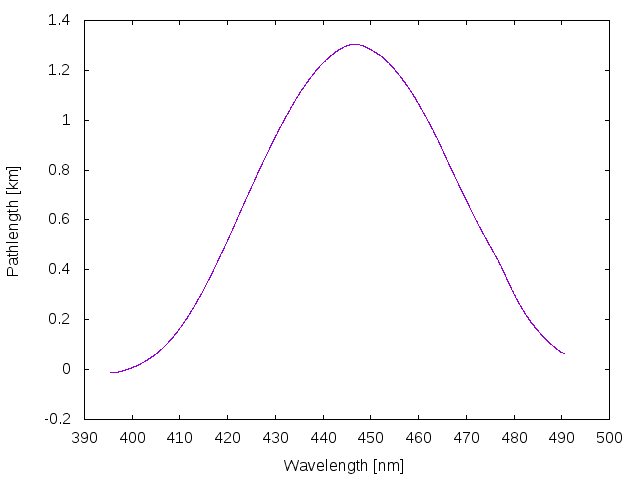
\includegraphics{../images/L0}}%
    \gplfronttext
  \end{picture}%
\endgroup

  \caption{Effective pathlength of the used EnviMeS CE-DOAS system.}
  \label{fig:pathlength}
\end{figure}

%%% Local Variables:
%%% mode: latex
%%% TeX-master: "../Bachelor"
%%% End:
